\begin{figure}
\centering
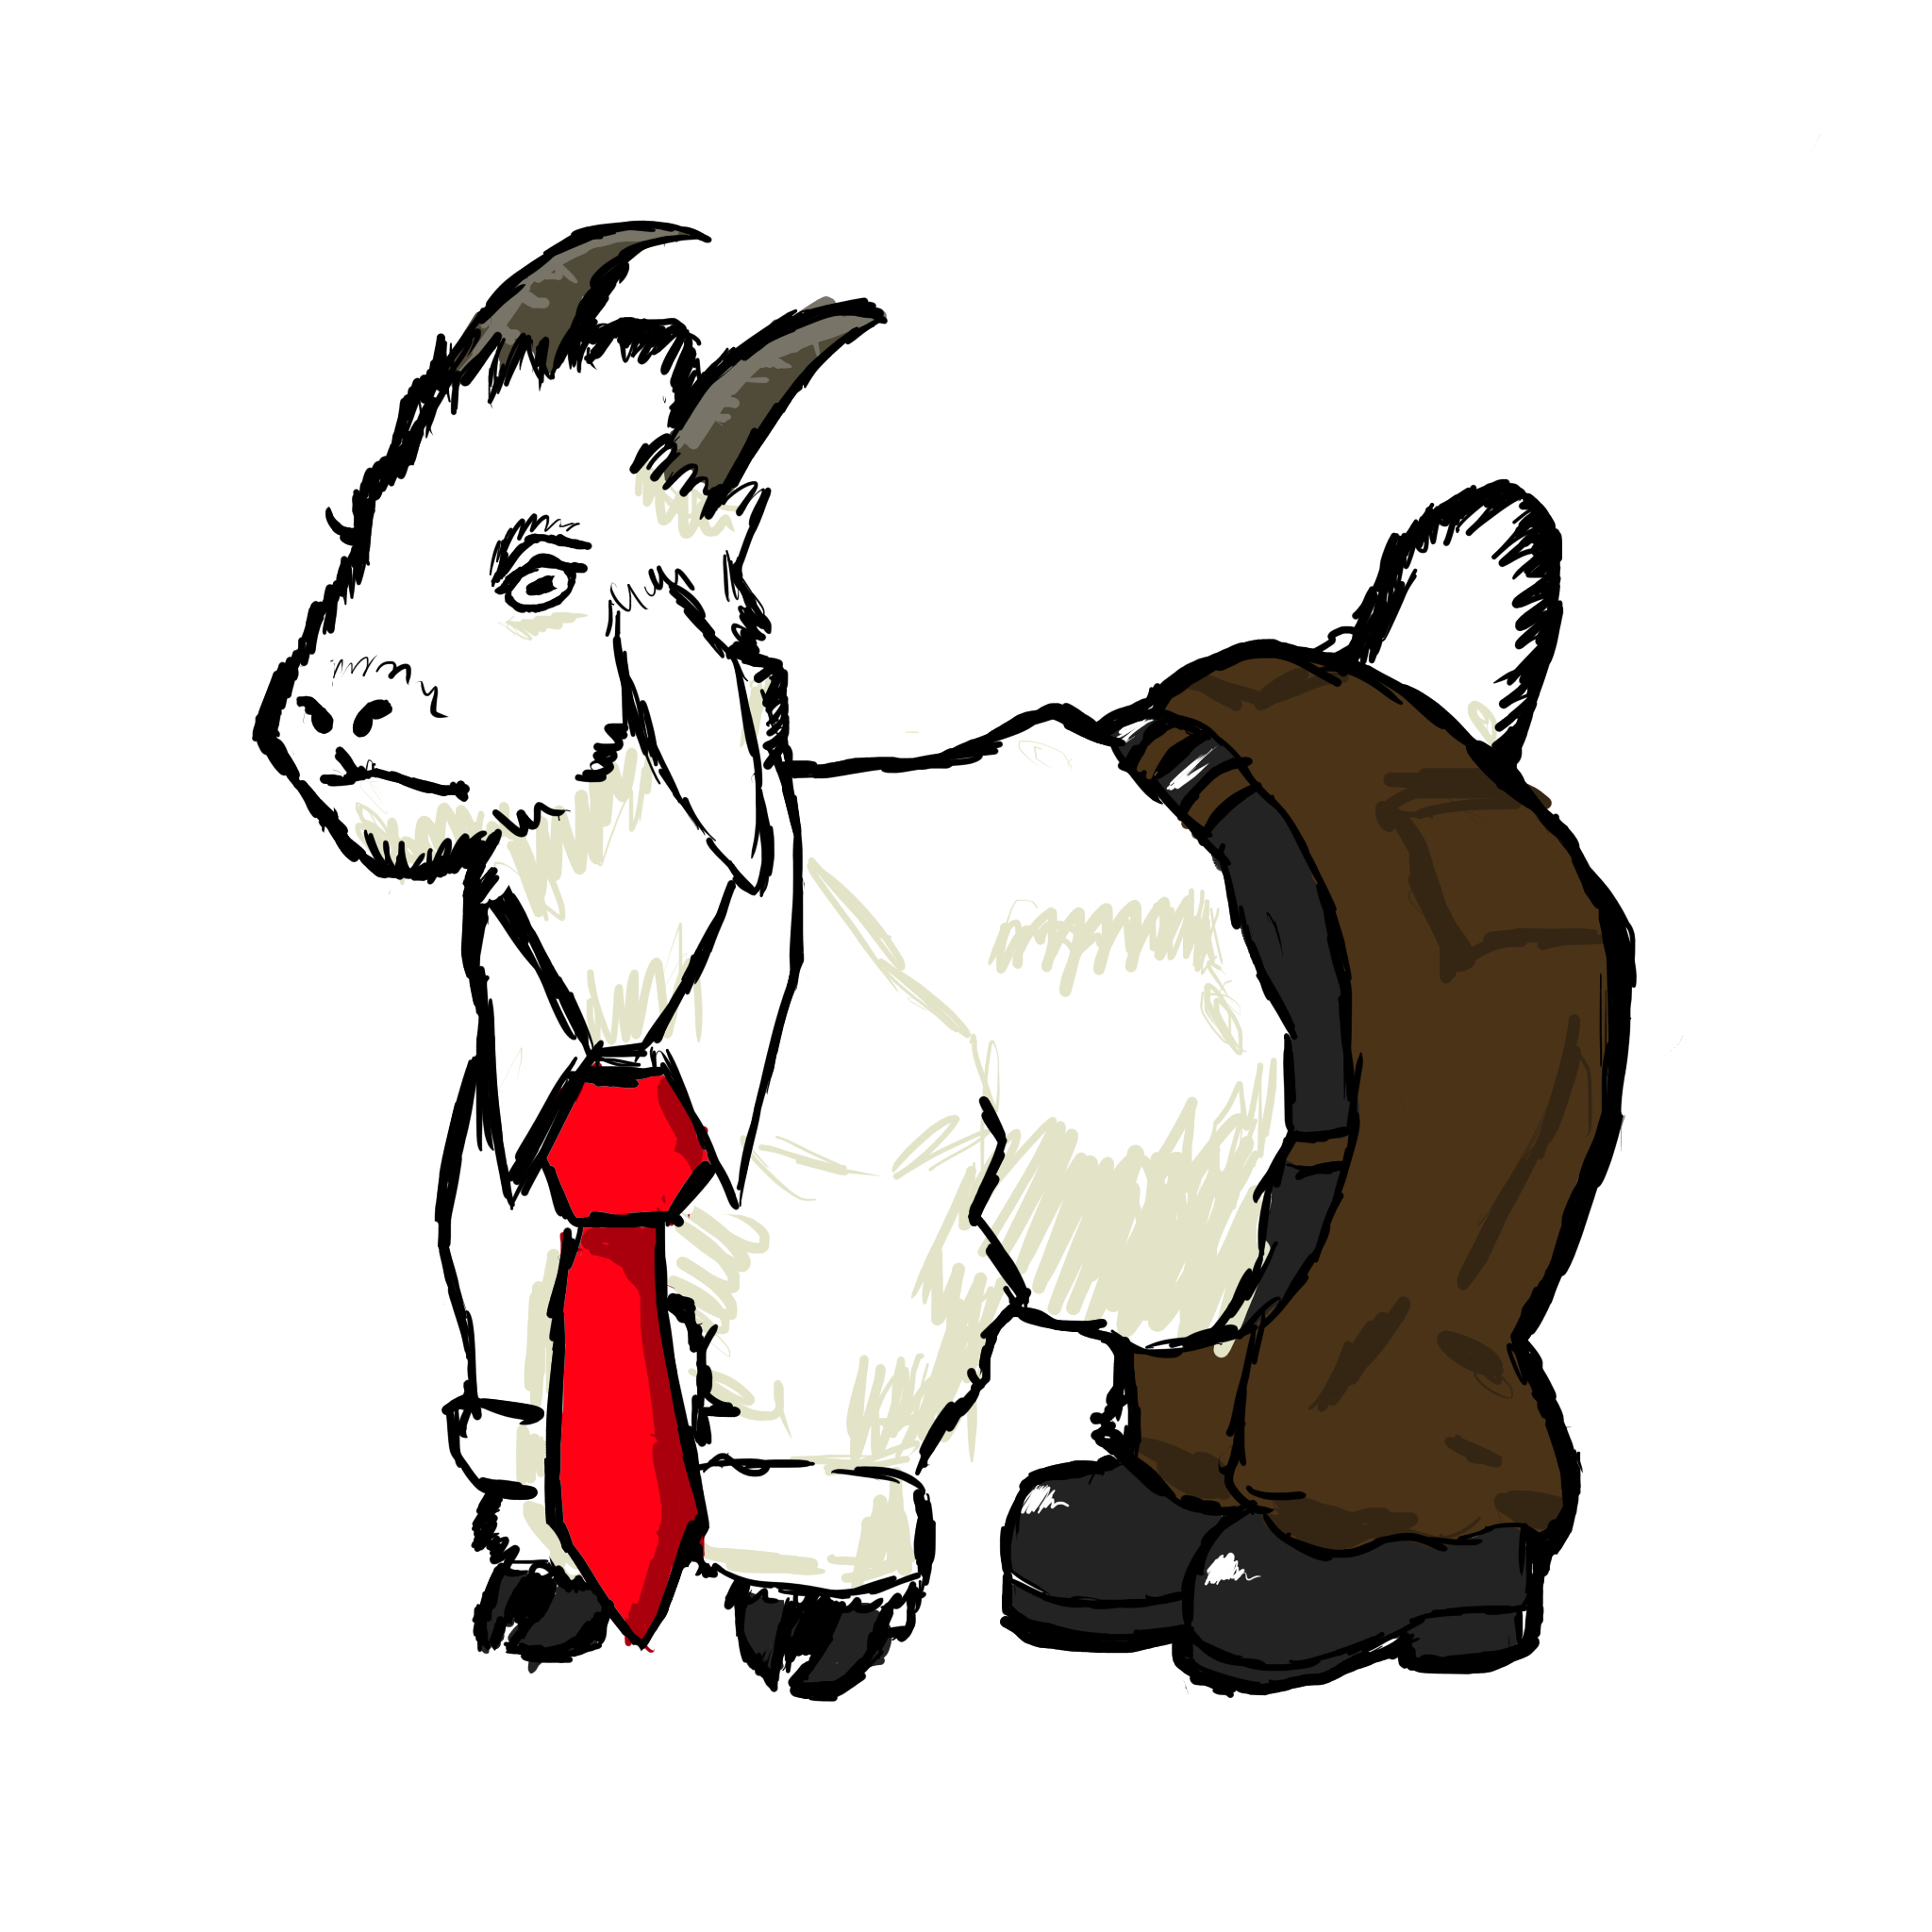
\includegraphics[width=3.5in,height=0.93in]{ECEWordMark-Tower_black.png}
\end{figure}

\maketitle

\newpage

%\begin{center}
%\bf{\underline{\color{blue} Preface}}
%\end{center}


%\begin{slshape} \color{blue}
\section*{Acknowledgements}

No-one has helped us significantly enough to deserve to be mentioned in the Acknowledgments.


%\newpage

%\section*{Preface}

%TBD.

%Requirements documents spring out of military/aerospace methods and are part of a formal process intended to minimize needed redesign.  These systems design methods are heavily front-loaded requiring extensive pre-design effort.  When properly exercised these methods can, and do, produce safe, effective systems that are on time and budget.  Requirements documents help with the so-called concurrent engineering process in that all aspects of the project are specified at the beginning of the project down to and including the kind of box that the system is going to be put in.  Concurrent engineering lessens the chances of unpleasant surprises late in the program.  Hearing things like, ``What do you mean it has to fit in a two inch cube?", six months into a program is frustrating and expensive.  There are less formal methodologies that demand less up front work, but while it is easy to relax the formal it is often hard to go the other way.
%\bigskip  

%Software developers often advocate design through methods like Extreme Programming or Agile.  Some pieces of these methods are quite useful, e.g. users stories, but as a crusty old design engineer I do not like an approach that uses near constant redesign as a design methodology.  When push comes to shove and lives are at stake, engineers will almost always choose a formal systems design methodology.
%\bigskip  

%Many people say that this formal style of engineering development is pass\'{e} and that newer, speedier, more flexible methods should be taught and used.  And yet they are unknowingly depending on these formal techniques every time they step onto an airplane.  To those who pine for the less formal methods I always ask the following question:

%\begin{quote}
%Would you fly on an airplane designed by the methods you advocate?
%\end{quote}

%The answer is seldom yes.

%\end{slshape}

%\newpage



%\begin{slshape}
%\color{blue}
%\section*{How to Use This Document}

%This document is divided into five major sections.  While specification document formats vary from group to group the format presented here is a good representation of what you will encounter in industrial specifications.  The sections of the document are:

%\begin{enumerate}
%	\item Scope
%	\item Applicable Documents
%	\item Stakeholder Requirements
%	\item Engineering Requirements
%	\item Verification of Requirements
%\end{enumerate}
%
%This document is not only intended to explain engineering specification documents and show the development of a specification through the use of a running example.  It also aims to help you produce a specification for your project.  In order to achieve this goal each section will be presented in three levels.  I will:
%
%\begin{enumerate}
%	\item Attempt to explain the reasons that the section exists and what data goes into that section.
%	\item Complete that section for the running example and annotate the example to make it more understandable.
%	\item Strongly suggest that you complete the section for your project.  When you see the symbol\vspace{.5cm} \StopSign\vspace{.5cm} it means you are going to get to produce something.
%\end{enumerate} 
%
%
%A skeleton template will be available in the same place that you found this document.  Fill out that skeleton template as you follow through this document.  You will quickly produce a specification in the least painful way I can think of.  Note that I didn't say pain free.  Sometimes thinking as hard as you need to think in engineering design just makes your head hurt.  
%
%
%\end{slshape}

\newpage

\begin{center} 
\Large{Signature Page}\\
\end{center}

\noindent \namesigdate{} \hfill \namesigdate{} \hfill \namesigdate{}

\newpage

\begin{center}
\Large{Revision History}\\
\end{center}

\begin{table}[h]
\centering
\begin{tabular}{|c|c|C{6cm}|c|c|}
\hline
\textbf{Revision} & \textbf{Description}& 
\textbf{Author} & \textbf{Date} & \textbf{Approval} \\
\hline
1 & Initial Revision & James and Braydan & Oct 24, 2018 &  \\
\hline
2 & & & & \\
\hline
3 & & & & \\
\hline
4 & & & & \\
\hline
5 & & & & \\
\hline
6 & & & & \\
\hline
7 & & & & \\
\hline
8 & & & & \\
\hline
9 & & & & \\
\hline
10 & & & & \\
\hline
\end{tabular}
\end{table}



%\begin{slshape}
%\color{blue}
%A simple hardware example will be used throughout this guide to illustrate the writing of a specification document.  The USU ECE Controls Lab needs a new power amplifier.  The requirements for its design follow the narrative in this document.
%\bigskip 
  
%From experience I know that I will not get it all right the first time.  If you find what you believe to be a mistake or omission, and can make a good case for why you feel that this is so, then I will revise the document and immortalize your name in the revision table.
%\end{slshape}
%\bigskip


\newpage

\clearpage\phantomsection\pdfbookmark{\contentsname}{toc} \tableofcontents

\raggedright


\newpage


\begin{center}
\Large{Specifications}
\end{center}

%\begin{python}%
%print ("Hello \LaTeX!")
%\end{python}%

%\begin{python}%
%TheFile = open('CourseInstructorSafety.tex')
%
%for eachLine in TheFile:
    %eachLine = eachLine.replace('\colorbox{yellow}','')
    %print(eachLine, end = '')
	%
%TheFile.close()
%\end{python}%